\documentclass{article}
\usepackage[utf8]{inputenc}
\usepackage[T5]{fontenc} % For Vietnamese support
\usepackage{vietnam} % Optional for better Vietnamese typesetting
\usepackage{graphicx}
\usepackage{hyperref}
\usepackage{booktabs} % For better tables
\usepackage{enumitem} % For customized lists
\usepackage{amsmath} % For math environments if needed
\usepackage{amssymb} % For \mathbb and other math symbols

 \usepackage{float}
\usepackage{algorithm}
\usepackage{algpseudocode}
\usepackage[numbers]{natbib}

\usepackage[a4paper, margin=1in]{geometry} % lề chuẩn 2.54 cm
\usepackage{times}                         % phông Times New Roman
\usepackage{setspace}                      % chỉnh giãn dòng
\setstretch{1.15}                          % giãn dòng 1.15
\setlength{\parindent}{15pt}               % thụt đầu dòng
\setlength{\parskip}{6pt}                  % khoảng cách giữa các đoạn
\usepackage{microtype}                     % cải thiện căn lề hai bên
 \usepackage{ragged2e}

 \usepackage{listings}
\usepackage{xcolor}

\lstset{
  language=Python,
  basicstyle=\ttfamily\small,
  backgroundcolor=\color{gray!10},
  frame=single,
  rulecolor=\color{black!30},
  keywordstyle=\color{blue!70}\bfseries,
  commentstyle=\color{green!40!black},
  stringstyle=\color{orange!70!black},
  showstringspaces=false,
  columns=fullflexible
    breaklines=false,
  breakatwhitespace=false
}

 
\title{Các Kỹ thuật Phân hoạch Lồi cho Hoạch định Chuyển động Robot}
\date{}

\begin{document} 
\raggedbottom
\sloppy
\justifying


\maketitle
\tableofcontents
\newpage


\section{Các Nguyên tắc Nền tảng của Phân hoạch Lồi}

\subsection{Định nghĩa}

\textbf{Phân hoạch lồi (Convex Decomposition)} là quá trình chia một hình học phức tạp (ví dụ: đa giác hoặc đa diện không lồi) 
thành một tập hợp các \textbf{vùng con lồi} sao cho hợp của các vùng này khôi phục lại toàn bộ hình ban đầu và 
các vùng con không chồng lấn nhau, ngoại trừ biên chung.  

Về mặt hình thức, với một miền hình học $P\subset\mathbb{R}^n$, 
một \textit{phân hoạch lồi} của $P$ là tập hợp $\{P_1, P_2, \dots, P_k\}$ sao cho:
\[
P = \bigcup_{i=1}^{k} P_i, \quad 
P_i \cap P_j = \partial P_i \cap \partial P_j \ \text{với mọi } i \ne j,
\]
và mỗi $P_i$ là một tập lồi.  
Mục tiêu là tìm tập phân hoạch này như là số lượng các vùng lồi tối thiểu, giảm thiểu phần chồng chéo hay chất lượng của vùng lồi được tạo ra (tránh quá "mảnh" hoặc "dài").


\subsection{Điều kiện Tồn tại Phân hoạch Lồi}

Nền tảng của nhiều thuật toán hoạch định chuyển động hiện đại dựa trên việc phân hoạch không gian cấu hình (configuration space) phức tạp thành một tập hợp các vùng lồi đơn giản hơn. 

Một câu hỏi cơ bản là: khi nào một phân hoạch như vậy tồn tại? Về mặt lý thuyết, điều kiện tồn tại khá rộng rãi. Đối với trường hợp phổ biến nhất trong hình học tính toán, bất kỳ đa giác đơn nào (đa giác không có cạnh tự cắt) đều có thể được phân hoạch thành một tập hợp các vùng lồi.\cite{keil1985}

$\Rightarrow$ Bởi thực tế là mọi đa giác đơn đều có thể được tam giác hóa, và mỗi tam giác là một tập lồi. Tuy nhiên, nó thường tạo ra một số lượng lớn các thành phần, làm cho nó không thực tế cho các ứng dụng hoạch định chuyển động hiệu quả.\cite{lien2006}

Khái niệm này được mở rộng ra ngoài các đa giác hai chiều. Bất kỳ tập lồi, đóng P nào trong không gian Euclid n-chiều đều có thể được phân hoạch thành các vùng con lồi, đóng nhỏ hơn.\cite{keil1985} Do đó, đối với các vấn đề thực tế trong lĩnh vực robot, câu hỏi quan trọng không phải là liệu một phân hoạch lồi có tồn tại hay không, mà là làm thế nào để tìm một phân hoạch hữu ích và hiệu quả về mặt tính toán.

\subsection{Phân loại Phương pháp Phân hoạch Lồi}
\label{sec:convex-decomposition-types}

Trong lĩnh vực hình học tính toán và hoạch định chuyển động, các phương pháp phân hoạch lồi thường được chia thành hai loại chính: 
\textbf{Phân hoạch Lồi Chính xác (Exact Convex Decomposition – ECD)} 
và 
\textbf{Phân hoạch Lồi Xấp xỉ (Approximate Convex Decomposition – ACD)}. 
Sự khác biệt giữa hai loại này phản ánh sự đánh đổi cơ bản giữa \textit{tính chính xác hình học} và \textit{hiệu quả tính toán}.

\subsubsection{Phân hoạch Lồi Chính xác (Exact Convex Decomposition – ECD)}

Phân hoạch Lồi Chính xác (ECD) là quá trình chia một hình dạng không lồi thành các \textbf{thành phần con hoàn toàn lồi}, 
không chồng lấn, sao cho hợp của chúng tái tạo lại chính xác hình dạng ban đầu. 
Mục tiêu thường là tối thiểu hóa số lượng vùng lồi.  

Tuy nhiên, ECD gặp hai thách thức lớn:
\begin{itemize}
    \item \textbf{Độ phức tạp tính toán cao:}  
    Bài toán tìm phân hoạch lồi tối thiểu đã được chứng minh là NP-hard đối với đa giác có lỗ, 
    nên không tồn tại thuật toán hiệu quả cho các trường hợp tổng quát.
    \item \textbf{Tính khả dụng hạn chế:}  
    Ngay cả khi tính toán được, ECD thường tạo ra số lượng vùng rất lớn, 
    khiến việc lưu trữ, xử lý và tối ưu hóa tiếp theo trở nên tốn kém.
\end{itemize}
Do đó, các phương pháp ECD chủ yếu mang tính lý thuyết, dùng làm chuẩn so sánh, 
trong khi hầu hết các ứng dụng thực tế trong robot và mô phỏng đều dựa vào các phương pháp xấp xỉ.

\subsubsection{Phân hoạch Lồi Xấp xỉ (Approximate Convex Decomposition – ACD)}

Trước những giới hạn của ECD, các phương pháp \textbf{Phân hoạch Lồi Xấp xỉ (ACD)} được phát triển để đạt sự cân bằng giữa độ chính xác và hiệu quả.  
ACD cho phép các thành phần không hoàn toàn lồi, mà chỉ “\textit{gần lồi}” trong một mức dung sai lõm $\tau$ do người dùng xác định.  
Triết lý cốt lõi của ACD là chấp nhận một \textbf{mức độ lõm nhỏ có kiểm soát} để đổi lấy:
\begin{itemize}
    \item \textbf{Hiệu quả tính toán cao hơn:} Các thuật toán ACD, chẳng hạn như phương pháp của Lien và Amato, chạy nhanh hơn nhiều so với ECD.
    \item \textbf{Giảm mạnh số lượng vùng:} Cho phép biểu diễn hình dạng với ít vùng lồi hơn, đơn giản hơn và dễ xử lý hơn.
    \item \textbf{Kiểm soát mức độ chi tiết:} Thông qua tham số $\tau$, người dùng có thể chọn giữa phân hoạch mịn (chính xác hơn) và phân hoạch thô (tổng quát hơn). 
\end{itemize}  


\section{Các Phương pháp Cốt lõi cho Phân hoạch Không gian Tự do}

Để giải quyết thách thức về tính toán của phân hoạch tối ưu, một số các phương pháp đã được phát triển. Dưới đây là một số phương pháp mà nhóm tìm được từ bài báo Motion Planning around Obstacles with Convex Optimization và một số phương pháp mở rộng thêm khác.

\subsection{Phân hoạch Lồi Xấp xỉ (ACD) của Đa giác} 

Phương pháp Approximate Convex Decomposition (ACD) giới thiệu một cách tiếp cận khác biệt cơ bản để quản lý sự phức tạp. Thay vì yêu cầu sự lồi hoàn hảo, nó cho phép các thành phần "lồi xấp xỉ" trong một dung sai do người dùng xác định, $\tau$.\cite{lien2006} Điều này thường dẫn đến các phân hoạch có ít thành phần hơn nhiều và phù hợp hơn với các đặc điểm cấu trúc nổi bật của đối tượng.

\subsubsection{Các Khái niệm Cơ bản trong Phân rã Lồi}
\label{sec:basic-concepts}

Phần này trình bày các khái niệm hình học cơ bản được sử dụng trong quá trình phân rã đa giác không lồi thành các vùng lồi. 
Các định nghĩa này đóng vai trò nền tảng cho các phương pháp đo độ lõm và các thuật toán phân hoạch ở các phần sau.

\begin{itemize}
    \item \textbf{Vỏ Lồi (Convex Hull – $H_P$):}  
    Vỏ lồi của một đa giác $P$ là \textbf{tập hợp lồi nhỏ nhất chứa toàn bộ đa giác} đó.  
    Trực quan, có thể hình dung vỏ lồi như một sợi dây chun được kéo căng bao quanh đa giác.  
    Một đa giác $P$ được gọi là \textbf{lồi} nếu và chỉ nếu nó trùng với vỏ lồi của chính nó, tức là:
    \[
    P = H_P.
    \]

    \item \textbf{Khía (Notches):}  
    Là các đỉnh của đa giác $P$ \textbf{không nằm trên vỏ lồi} $H_P$.  
    Về mặt hình học, đây là những đỉnh có \textbf{góc trong lớn hơn $180^\circ$}.  
    Các khía biểu hiện các đặc trưng lõm (concave features) trên biên của đa giác.

    \item \textbf{Cầu (Bridges):}  
    Là các cạnh của vỏ lồi $\partial H_P$ nối hai đỉnh không liền kề của biên ngoài $\partial P_0$.  
    Về mặt toán học, tập hợp các cầu được định nghĩa:
    \[
    \text{BRIDGES}(P) = \partial H_P \setminus \partial P.
    \]
    Mỗi cầu “bắc qua” một vùng lõm của đa giác.

    \item \textbf{Túi (Pockets):}  
    Là các \textbf{chuỗi cạnh liên tiếp} của biên đa giác $\partial P$ không thuộc về vỏ lồi $\partial H_P$.  
    Về mặt toán học:
    \[
    \text{POCKETS}(P) = \partial P \setminus \partial H_P.
    \]
    Mỗi túi tương ứng với một “vịnh lõm” (concave bay) trên đường biên của đa giác.
\end{itemize}

\begin{figure}[H]
    \centering
    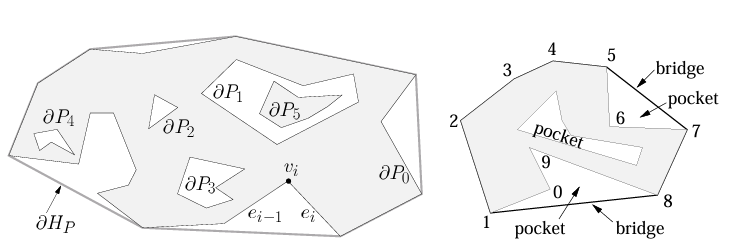
\includegraphics[width=0.7\linewidth]{imgs/ACD-5.png}
    % \caption{Enter Caption}
\end{figure}

\subsubsection{Ý tưởng và Chi tiết Thuật toán}



Thuật toán là một chiến lược chia để trị đệ quy\cite{lien2006}:
\begin{enumerate}
\item Đo độ lõm: Xác định đặc điểm không lồi (một "notch" hay đỉnh lõm) quan trọng nhất trong đa giác. Đây là điểm có độ lõm lớn nhất. Tùy theo từng trường hợp mà ta có thể sử dụng các thước đo độ lõm khác nhau, cách để tính những thước đo độ lõm nãy sẽ được giới thiệu rõ hơn ở phần ~\ref{sec:MEASURING-CONCAVITY}


\item Kiểm tra Dung sai: Nếu độ lõm tối đa đo được nhỏ hơn $\tau$, quá trình kết thúc đối với thành phần đó.

\item Giải quyết Đỉnh lõm: Nếu độ lõm vượt quá $\tau$, một đường cắt được thêm vào để giải quyết đỉnh lõm, chia đa giác thành hai thành phần mới (hoặc hợp nhất một lỗ).

\begin{figure}[H]
    \centering
    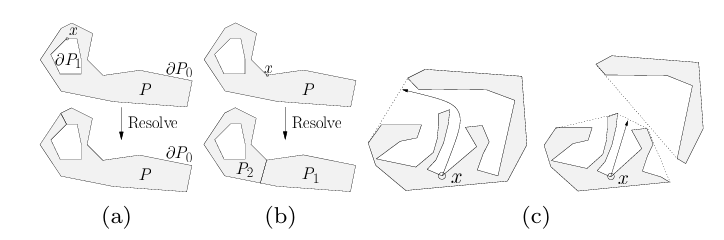
\includegraphics[width=1\linewidth]{imgs/ACD-3.png}
    \caption{%
        (a) Nếu $x \in \partial P_i > 0$, hàm \texttt{Resolve} \textbf{gộp} biên $\partial P_i$ vào đa giác $P_0$.
        (b) Nếu $x \in \partial P_0$, hàm \texttt{Resolve} \textbf{tách} đa giác $P$ thành hai đa giác $P_1$ và $P_2$.
        (c) \textbf{Độ lõm} tại điểm $x$ thay đổi sau khi đa giác được phân rã.%
    }
\end{figure}

\item Đệ quy: Quá trình được áp dụng đệ quy cho các thành phần mới.

\begin{figure}[H]
    \centering
    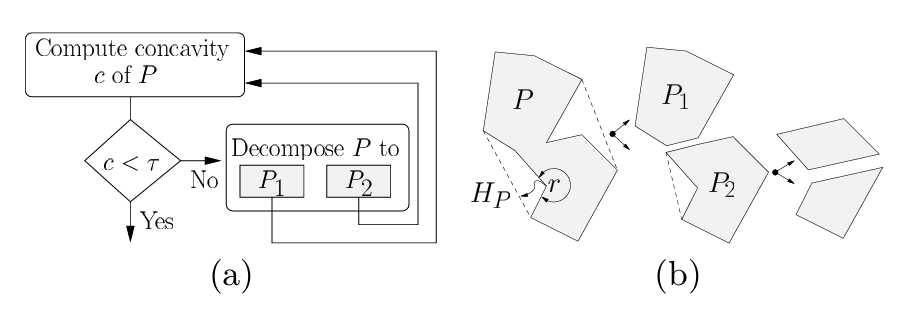
\includegraphics[width=0.5\linewidth]{imgs/ACD-1.png}
    \caption{Quá trình đệ quy tiếp tục cho đến khi đạt đến giới hạn độ lõm đầu vào của người dùng $\tau$.}
\end{figure}

\end{enumerate}

\subsubsection{Các Thước đo Độ lõm}
\label{sec:MEASURING-CONCAVITY}

Chất lượng của phân hoạch phụ thuộc rất nhiều vào \textbf{cách đo độ lõm} của các đỉnh trong đa giác không lồi. Các phương pháp đo độ lõm phổ biến bao gồm:

\begin{itemize}
    \item \textbf{Độ lõm Đường thẳng (Straight-Line Concavity – SL-Concavity)}:  
    Là khoảng cách Euclid từ một đỉnh trong \textit{túi} (pocket) đến \textit{cầu nối} (bridge) liên kết của nó — thường là một cạnh thuộc bao lồi của đa giác.  
    Phương pháp này rất nhanh, nhưng \textbf{không đảm bảo tính đơn điệu}, có thể khiến một số đặc trưng lõm quan trọng bị bỏ sót.

    \begin{figure}[H]
        \centering
        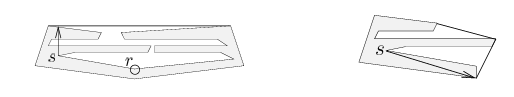
\includegraphics[width=0.7\linewidth]{imgs/ACD-2.png}
        \caption{%
            Giả sử $r$ là điểm lõm có độ lõm lớn nhất. 
            Sau khi giải quyết (resolve) $r$, độ lõm của $s$ tăng lên. 
            Nếu $\text{concave}(r) < \tau$, vùng $s$ sẽ không bao giờ được xử lý, 
            ngay cả khi $\text{concave}(s)$ lớn hơn $\tau$.%
        }
        \label{fig:nonmonotonic-concavity}
    \end{figure}

    \item \textbf{Độ lõm Đường đi Ngắn nhất (Shortest Path Concavity – SP-Concavity)}:  
    Là \textbf{chiều dài đường đi ngắn nhất} từ một đỉnh trong túi đến cầu nối tương ứng, với điều kiện đường đi đó phải nằm hoàn toàn trong túi.  
    Phương pháp này chậm hơn SL-Concavity nhưng \textbf{đảm bảo tính đơn điệu}: độ lõm của các đỉnh giảm dần sau mỗi lần phân rã, 
    giúp đảm bảo rằng tất cả các đặc điểm lõm quan trọng cuối cùng sẽ được xử lý.  
    (Xem chi tiết trong Phần~\ref{sec:SP-Concavity}.)

    \item \textbf{Độ lõm Lai (Hybrid Concavity – H-Concavity)}:  
    Một giải pháp trung gian thực tiễn — sử dụng SL-Concavity nhanh làm mặc định và chỉ chuyển sang SP-Concavity khi \textbf{phát hiện khả năng không đơn điệu}. Bằng cách thêm bước kiểm tra \textit{nguy cơ tiềm ẩn} bằng cách so sánh $n_\beta$ và $n_i$; nếu tồn tại $n_i \cdot n_\beta < 0$, biên túi bị đảo hướng — dấu hiệu của túi phức tạp mà SL-Concavity có thể thất bại.

    \begin{figure}[H]
        \centering
        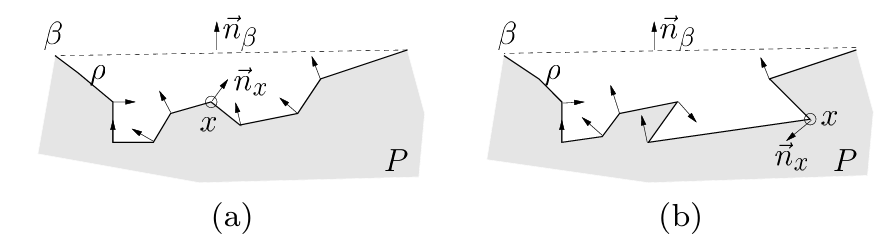
\includegraphics[width=0.5\linewidth]{imgs/ACD-6.png}
        \caption{Độ lõm SL có thể xử lý được túi trong (a) một cách chính xác vì không có hướng chuẩn nào của các đỉnh trong túi ngược với hướng chuẩn của cầu. Tuy nhiên, túi trong (b) có thể dẫn đến độ lõm giảm không đơn điệu.}
    \end{figure}
   
\end{itemize}

\subsubsection{Đặc tính của Thuật toán}

\begin{itemize}
\item Loại thuật toán: Đây là một phương pháp xấp xỉ theo định nghĩa. Một phân hoạch với $\tau=0$ là một phân hoạch lồi chính xác.
\item Độ phức tạp thời gian: $O(n r^2)$, trong đó $n$ là số đỉnh và $r$ là số đỉnh lõm.\cite{lien2006} Điều này nhanh hơn các thuật toán phân hoạch chính xác tối ưu cho đa giác không có lỗ.
\end{itemize}



\subsection{Iterative Regional Inflation by Semi-Definite Programming (IRIS)}

Thuật toán Iterative Regional Inflation by Semidefinite Programming (IRIS) thay vì cố gắng bao phủ toàn bộ không gian tự do cùng một lúc, nó đặt ra câu hỏi: "Với một điểm 'mầm' (seed) ban đầu, vùng lồi lớn nhất của không gian tự do mà tôi có thể tìm thấy xung quanh nó là gì?".  Tức sau khi chạy xong giải thuật output của ta là một vùng lồi lớn nhất có thể của thuật toán từ 1 seed point cho trước.

\subsubsection{Ý tưởng và Chi tiết Thuật toán}

IRIS là một quy trình tối ưu hóa lặp đi lặp lại gồm 4 bước:
\begin{enumerate}
\item \textbf{Khởi tạo}: Thuật toán sẽ tạo ra một hình elip ban đầu là một hình cầu rất nhỏ có tâm chính là điểm mầm (seed point).
\item \textbf{Tìm Siêu phẳng Phân cách (QP)}: 

\begin{figure}[!htp]
    \centering
    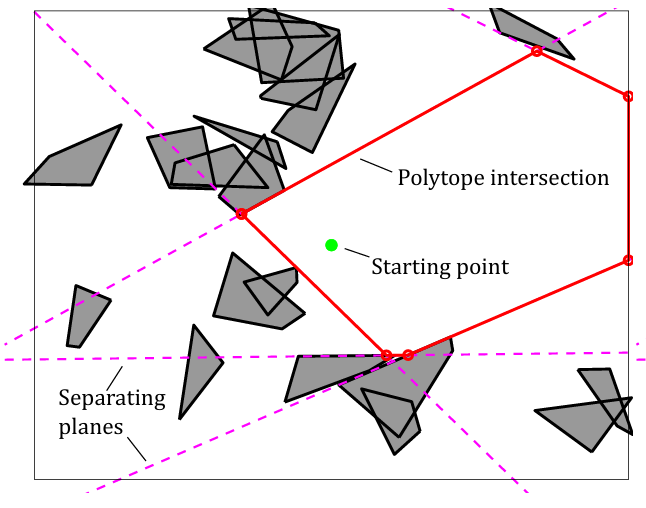
\includegraphics[width=0.5\linewidth]{imgs/iris_algo_1.png}
    \caption{Siêu phẳng Phân cách}
\end{figure}

Đối với ellipsoid hiện tại, thuật toán tìm điểm gần nhất trên mỗi chướng ngại vật. Sau đó, nó xây dựng các siêu phẳng phân cách ellipsoid khỏi các chướng ngại vật này. Mỗi siêu phẳng tiếp tuyến với một phiên bản mở rộng của ellipsoid và đi qua điểm gần nhất trên chướng ngại vật tương ứng. Việc tìm điểm gần nhất trên mỗi chướng ngại vật lồi được xây dựng như một bài toán Quy hoạch Toàn phương (Quadratic Program - QP). Để giữ cho bài toán tối ưu hóa tiếp theo có quy mô nhỏ, các siêu phẳng thừa (những siêu phẳng không xác định biên của vùng lồi kết quả) sẽ được loại bỏ.

\textbf{Bước 2.1}. Tìm điểm gần nhất trên obstacle đến hình elip hiện tại
\begin{itemize}
\item \textbf{Biến đổi không gian (Từ không gian Ellipsoid sang không gian Quả cầu đơn vị)}  

Việc tính toán khoảng cách đến một ellipsoid là phức tạp. Tuy nhiên, tính khoảng cách đến một quả cầu đơn vị tại gốc tọa độ thì lại rất đơn giản. Ý tưởng ở đây là biến đổi toàn bộ không gian sao cho ellipsoid trở thành một quả cầu đơn vị.

\begin{itemize}
    \item Một ellipsoid $E$ được định nghĩa là ảnh của một quả cầu đơn vị $\tilde{E}$ qua phép biến đổi affine:
    \[
    x = C\tilde{x} + d.
    \]
    \item Sử dụng phép biến đổi ngược:
    \[
    \tilde{x} = C^{-1}(x - d),
    \]
    để ánh xạ mọi điểm trở lại “không gian quả cầu đơn vị”.
    \item Trong không gian mới này, ellipsoid trở thành quả cầu đơn vị $\tilde{E}$ tại gốc tọa độ, và mỗi chướng ngại vật $l_j$ cũng bị biến đổi (méo đi) thành một đối tượng mới $\tilde{l_j}$.
\end{itemize}
\end{itemize}

\textbf{Bước 2.2}: Tìm điểm gần nhất bằng Quy hoạch Toàn phương (QP)

Bây giờ, bài toán tìm điểm trên chướng ngại vật $l_j$ gần ellipsoid $E$ nhất tương đương với việc tìm điểm trên chướng ngại vật đã biến đổi $\tilde{l_j}$ gần gốc tọa độ nhất.  

Bài toán này được xây dựng dưới dạng một bài toán \textit{Quy hoạch Toàn phương} (Quadratic Program - QP):

\[
\begin{aligned}
    &\underset{\tilde{x} \in \mathbb{R}^n,\, w \in \mathbb{R}^m}{\text{minimize}} && \|\tilde{x}\|^2 \\
    &\text{subject to} 
    && 
    \begin{cases}
        [\, \tilde{v}_{j,1} \; \tilde{v}_{j,2} \; \cdots \; \tilde{v}_{j,m} \,]\, w = \tilde{x}, \\
        \sum_{i=1}^{m} w_i = 1, \\
        w_i \ge 0, \quad i = 1,\dots,m.
    \end{cases}
\end{aligned}
\]

\noindent
Về bản chất, ta đang tìm một điểm $\tilde{x}$ là \textbf{tổ hợp lồi} của các đỉnh đã biến đổi $\tilde{v}_{j,k}$ sao cho khoảng cách của $\tilde{x}$ đến gốc tọa độ là nhỏ nhất.  

\textbf{Bước 2.3}. Xác định mặt phẳng tiếp tuyến của ellipsoid tại điểm tiếp xúc

Sau khi tìm được điểm \(x^*\) gần nhất, ta xây dựng mặt phẳng tiếp tuyến với ellipsoid tại điểm đó.  
Ellipsoid được mô tả bằng biểu thức nghịch đảo:

\[
E = \{\, x \mid (x - d)^{\top} C^{-1} C^{-\top} (x - d) \le 1 \,\}.
\]

Vector pháp tuyến của ellipsoid tại \(x^*\) được xác định bởi gradient:

\[
a_j = \nabla_x \big[(x - d)^{\top} C^{-1} C^{-\top} (x - d)\big]_{x = x^*}
     = 2C^{-1}C^{-\top}(x^* - d).
\]

Vì mặt phẳng tiếp tuyến đi qua \(x^*\), ta có:

\[
b_j = a_j^{\top}x^*.
\]

Khi đó, phương trình mặt phẳng tiếp tuyến là:
\[
a_j^{\top}x = b_j,
\]
được thêm vào như một \textbf{ràng buộc tuyến tính} trong tập khả thi của thuật toán IRIS.  
Mặt phẳng này đảm bảo ellipsoid mở rộng tối đa nhưng không giao với chướng ngại vật.

\textbf{Bước 2.4}. Lặp lại với tất cả các obstacles trong không gian. Ta sẽ có được một tập các siêu phẳng để tạo thành một vùng lồi đa giác.

\newpage
\item \textbf{Tìm Ellipsoid Nội tiếp Cực đại (SDP)}: Giao của các nửa không gian được xác định bởi các siêu phẳng tạo thành một đa diện lồi (polytope). Thuật toán sau đó tìm ellipsoid có thể tích lớn nhất có thể nội tiếp trong đa diện này. 

\begin{figure}[!htp]
    \centering
    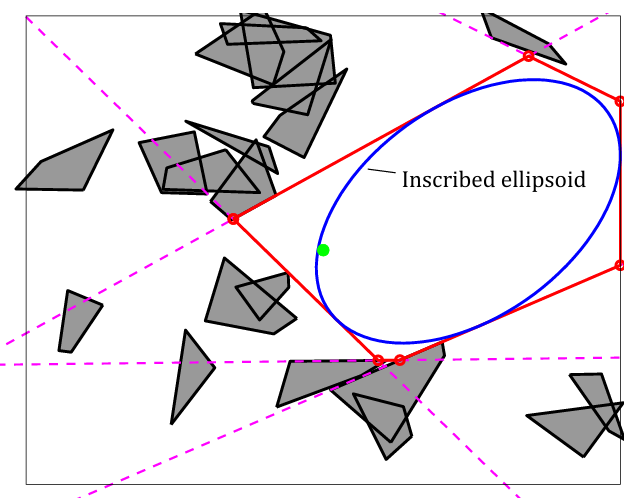
\includegraphics[width=0.5\linewidth]{imgs/iris_2.png}
    \caption{Ellipsoid Nội tiếp Cực đại}
\end{figure}

Bài toán này tìm \textbf{ellipsoid có thể tích lớn nhất} nằm gọn trong một đa diện lồi \( P \):
\begin{equation}
    P = \{x \in \mathbb{R}^n \mid A x \leq b\}.
\end{equation}

Ellipsoid được định nghĩa là \(\mathcal{E}\), với \(d\) là tâm và ma trận \(C\) xác định hình dạng:
\begin{equation}
    \mathcal{E} = \{C\tilde{x} + d \mid \|\tilde{x}\|_2 \leq 1\}.
\end{equation}

Thể tích của ellipsoid tỉ lệ với \(\det(C)\).

Để tìm ellipsoid lớn nhất nội tiếp trong \(P\), ta giải bài toán tối ưu lồi sau:
\begin{equation}
\begin{aligned}
    \underset{C,d}{\text{maximize}} \quad & \log \det C \\
    \text{subject to} \quad & \|a_i^{\top} C\|_2 + a_i^{\top} d \leq b_i, \quad \forall i = 1, \ldots, N, \\
    & C \succ 0.
\end{aligned}
\end{equation}

\noindent
\textbf{Mục tiêu:} Cực đại hoá \(\log \det C\) để tối đa hoá thể tích ellipsoid. \\[4pt]
\textbf{Ràng buộc:} Đảm bảo mọi điểm của ellipsoid đều nằm trong đa diện \(P\).



\item \textbf{Lặp lại}: Ellipsoid mới, lớn hơn này được sử dụng làm điểm khởi đầu cho vòng lặp tiếp theo. Quá trình này hội tụ khi thể tích của ellipsoid ngừng tăng một cách đáng kể, trả về một đa diện lồi lớn và ellipsoid nội tiếp của nó.
\end{enumerate}

\begin{figure}[!htp]
    \centering
    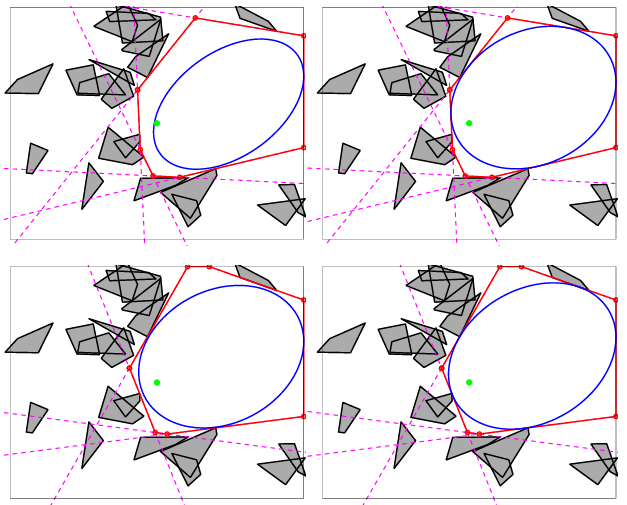
\includegraphics[width=0.5\linewidth]{imgs/iris-3.png}
    \caption{Lặp lại}
\end{figure}

\newpage
\subsubsection{Đặc tính của Thuật toán}

\begin{itemize}
\item Loại thuật toán: IRIS là một phương pháp xấp xỉ để bao phủ toàn bộ không gian tự do. Một lần chạy duy nhất chỉ tạo ra một vùng lồi. Để có được một lớp phủ hoàn chỉnh, cần phải chạy thuật toán nhiều lần với các điểm mầm khác nhau.
\item Độ phức tạp thời gian: IRIS thường hội tụ qua 4-8 vòng lặp. Thời gian tính toán của mỗi vòng lặp bằng thời gian tìm các mặt phẳng phân cách cộng với thời gian tính toán ellipses nội tiếp. Trong khi thời gian giải ellipses (SDP) gần như không đổi (constant) nhờ vào việc loại bỏ các siêu phẳng thừa thì thời gian tính các siêu phẳng phân cách lại tăng tuyến tính theo số lượng các obstacles.  
\begin{figure}[!htp]
    \centering
    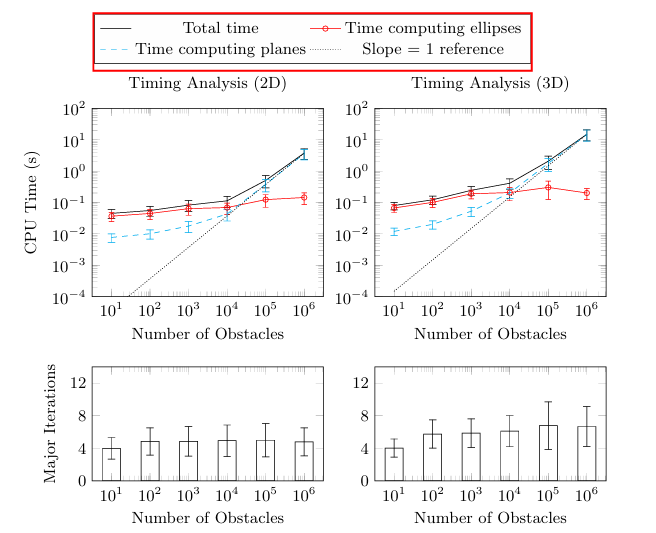
\includegraphics[width=0.5\linewidth]{imgs/time-iris.png}
    \caption{Độ phức tạp thời gian}
\end{figure}

\item Xử lý Vật cản không lồi:
\begin{itemize}
\item Chướng ngại vật trong không gian work space: Thuật toán IRIS ban đầu giả định các chướng ngại vật là lồi, đây cũng là một nhược điểm lớn nhất của thuật toán này. Để đảm bảo các obstacles là lồi, ta thường phải tiền xử lý bằng cách bao lồi  các chướng ngại vật không lồi\cite{DeitsTedrake2014}. Ngoài ra cách tiếp cận tiêu chuẩn cho các chướng ngại vật không lồi là phân hoạch chúng thành một tập hợp các mảnh lồi trước khi chạy IRIS (tức tăng số lượng obtacles của không gian lên). Điều này khả thi vì IRIS có khả năng mở rộng hiệu quả với số lượng lớn chướng ngại vật. 

\item Chướng ngại vật trong không gian cấu hình (Configuration Space): Đối với các robot có động học phức tạp, nơi các chướng ngại vật trong không gian cấu hình được định nghĩa một cách ẩn ý và không lồi, các phần mở rộng như IRIS-NP và C-IRIS được sử dụng. Đặc biệt, bài báo "Motion Planning around Obstacles with Convex Optimization" sử dụng một triển khai có tên là IrisInConfigurationSpace trong thư viện Drake cho ví dụ về cánh tay robot.\cite{motionplanning2022} Phần mở rộng này sử dụng lập trình phi tuyến (nonlinear programming) để xử lý hình học phức tạp của không gian cấu hình.
\end{itemize}
\end{itemize}

\subsection{Gieo mầm Tự động qua Lớp phủ Clique Khả kiến (VCC)}

Thuật toán Visibility Clique Cover (VCC) giải quyết trực tiếp một hạn chế chính của IRIS: nhu cầu về các điểm mầm tốt.$^5$ Việc lấy mầm ngẫu nhiên là không hiệu quả. VCC tự động hóa quá trình này bằng cách trước tiên tìm hiểu cấu trúc toàn cục của không gian tự do và sau đó đặt các điểm mầm một cách chiến lược vào các khu vực có khả năng mở rộng lớn.

\subsubsection{Ý tưởng và Chi tiết Thuật toán}

Quy trình VCC bao gồm bốn bước chính \cite{vcc2023}:
\begin{enumerate}
\item Lấy mẫu \& Xây dựng Đồ thị Khả kiến (Visibility Graphs): Thuật toán lấy mẫu $n$ điểm ngẫu nhiên trong không gian cấu hình tự do ($C_{free}$). Các điểm này tạo thành các đỉnh của một đồ thị khả kiến (visibility graph)\footnote{\textit{Visibility graph} là đồ thị trong đó các đỉnh biểu diễn vị trí (hoặc đỉnh chướng ngại vật), và có cạnh nối giữa hai đỉnh nếu đoạn thẳng nối chúng nằm hoàn toàn trong không gian tự do.}
. Một cạnh tồn tại giữa hai đỉnh nếu đoạn thẳng nối hai điểm tương ứng hoàn toàn nằm trong không gian tự do (tức là không va chạm).

\begin{figure}[H]
    \centering
    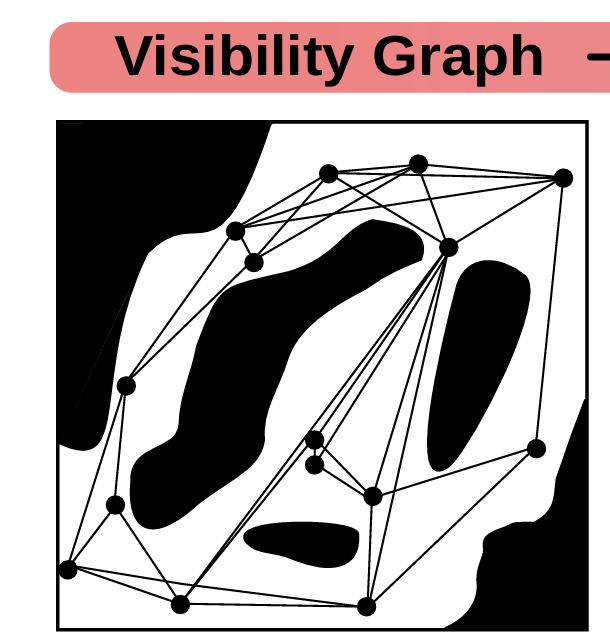
\includegraphics[width=0.5\linewidth]{imgs/VCC-1.png}
    \caption{Lấy mẫu \& Xây dựng Đồ thị Khả kiến (Visibility Graphs)}
\end{figure}

\item Tìm Lớp phủ Clique: Thuật toán tìm một tập hợp các clique lớn (đồ thị con đầy đủ) trong đồ thị khả kiến. Ý tưởng cốt lõi là một tập hợp các điểm mà tất cả đều "nhìn thấy" nhau có khả năng nằm trong cùng một vùng lồi\footnote{Nếu hai điểm có thể nhìn thấy nhau, điều đó ngụ ý rằng con đường thẳng nhất giữa chúng là an toàn. Đây là khối xây dựng cơ bản để hiểu và xấp xỉ các vùng lồi trong.}. Điều này được thực hiện một cách tham lam bằng cách giải lặp đi lặp lại bài toán MAXCLIQUE (tìm clique lớn nhất), được xây dựng dưới dạng một bài toán Integer Linear Programming - ILP.

\begin{figure}[H]
    \centering
    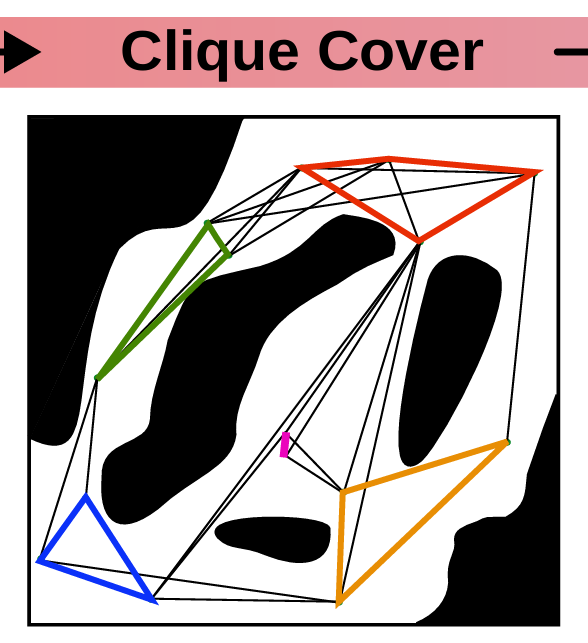
\includegraphics[width=0.5\linewidth]{imgs/VCC-2.png}
    \caption{Tìm Lớp phủ Clique}
\end{figure}

\item Khởi tạo Ellipsoid: Đối với mỗi clique được tìm thấy, thuật toán tính toán ellipsoid có thể tích nhỏ nhất bao quanh tất cả các điểm trong clique đó. Ellipsoid này cung cấp một tâm (điểm mầm) và các trục chính (hình dạng ban đầu) cho bước lấp đầy tiếp theo.

\begin{figure}[H]
    \centering
    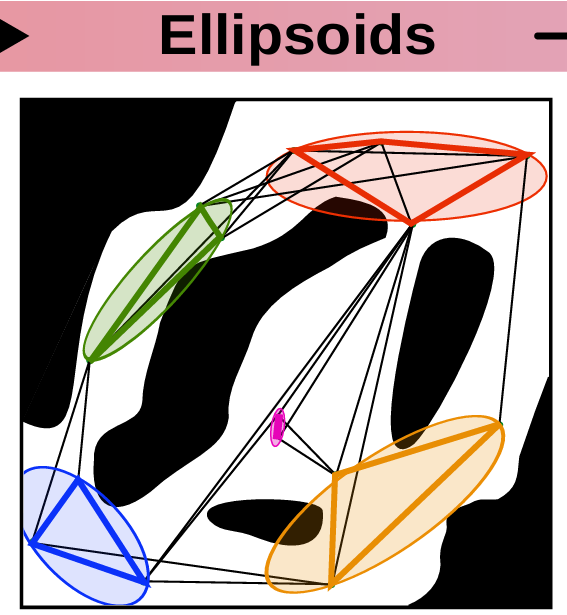
\includegraphics[width=0.5\linewidth]{imgs/VCC-3.png}
    \caption{Khởi tạo Ellipsoid}
\end{figure}

\item Lấp đầy thành Đa diện: Tâm và hình dạng của mỗi ellipsoid được sử dụng để khởi tạo một vòng lặp duy nhất của thuật toán lấp đầy tương tự IRIS. Điều này hiệu quả hơn IRIS tiêu chuẩn vì ellipsoid ban đầu đã được "thông báo" về hình học cục bộ, thường loại bỏ sự cần thiết của nhiều vòng lặp tốn kém.$^5$

\begin{figure}[H]
    \centering
    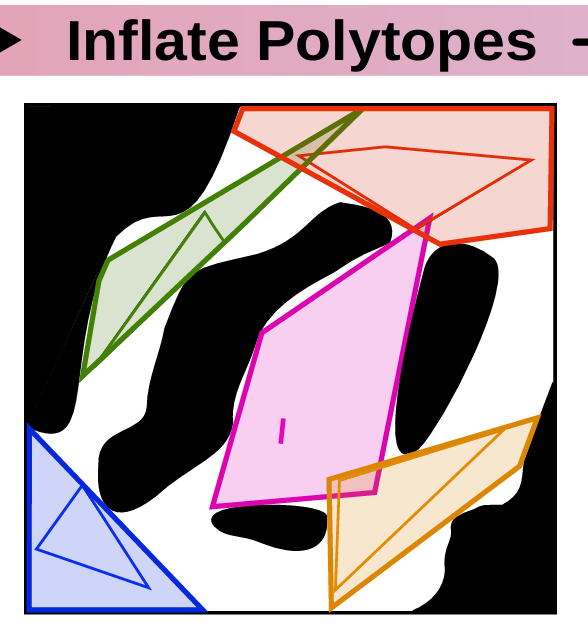
\includegraphics[width=0.45\linewidth]{imgs/VCC-4.png}
    \caption{Lấp đầy thành Đa diện}
\end{figure}

\item Lặp lại và Hội tụ: Quá trình này được lặp lại cho đến khi đạt được độ phủ đủ bằng cách lấy mẫu mới từ không gian trống còn lại và lặp lại các bước trước đó.


\begin{figure}[H]
    \centering
    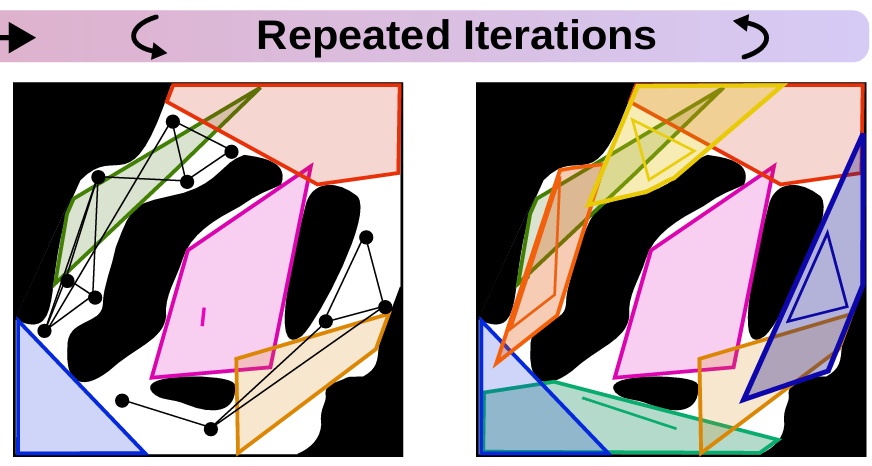
\includegraphics[width=0.5\linewidth]{imgs/VCC-5.png}
    \caption{Lặp lại}
\end{figure}

\end{enumerate}

\subsubsection{Đặc tính và Tính tối ưu}

\begin{itemize}
\item Loại thuật toán: VCC là một phương pháp xấp xỉ. Chất lượng của lớp phủ được đo bằng tỷ lệ phần trăm thể tích của $C_{free}$ được bao phủ bởi hợp của các đa diện kết quả.$^5$
\item Mục tiêu Tối ưu: Thuật toán nhằm tìm một lớp phủ lồi xấp xỉ $\alpha$ ($\alpha$-approximate convex cover) với số lượng vùng tối thiểu. Nó sử dụng bài toán lớp phủ clique tối thiểu (minimum clique cover) như một bài toán tương tự rời rạc cho bài toán lớp phủ lồi tối thiểu.\cite{vcc2023}
\item Phương pháp: Đây là một cách tiếp cận lai ghép giữa hình học và ILP.
\item Xử lý Không gian không lồi: VCC không phụ thuộc vào hình dạng của chướng ngại vật vì nó dựa vào một bộ kiểm tra va chạm chung để kiểm tra khả kiến và sau đó sử dụng một thuật toán lấp đầy cơ bản (như IRIS-NP) có thể xử lý các không gian cấu hình không lồi.\cite{vcc2023}
\end{itemize}

\section{Ứng dụng trong "Motion Planning around Obstacles with Convex Optimization"}

Bài báo "Motion Planning around Obstacles with Convex Optimization" giới thiệu một phương pháp hoạch định chuyển động mạnh mẽ dựa trên khuôn khổ Graphs of Convex Sets (GCS). Sự thành công của phương pháp này phụ thuộc trực tiếp vào sự tồn tại của một phân hoạch lồi hiệu quả của không gian tự do.

\subsection{Vai trò của Phân hoạch trong Khuôn khổ GCS}

Khuôn khổ GCS yêu cầu không gian tự do phải được phân hoạch trước thành một tập hợp các vùng lồi. Các vùng này không chỉ đơn thuần là các ràng buộc hình học; chúng trở thành các khối xây dựng cơ bản của bài toán tối ưu hóa. Mỗi vùng lồi tương ứng với một đỉnh trong đồ thị $G$ của công thức GCS.\cite{motionplanning2022}

Bộ hoạch định sau đó tìm một đường đi ngắn nhất qua đồ thị các tập hợp này, đồng thời tối ưu hóa cả chuỗi rời rạc các vùng cần đi qua và các đoạn quỹ đạo liên tục trong mỗi vùng.  Do đó, chất lượng, số lượng và kích thước của các vùng lồi được cung cấp bởi thuật toán phân hoạch có ảnh hưởng trực tiếp và sâu sắc đến hiệu suất và chất lượng giải pháp của bộ hoạch định GCS. Một phân hoạch kém (ví dụ, quá nhiều vùng nhỏ) sẽ dẫn đến một đồ thị lớn, phức tạp và một bài toán tối ưu hóa khó khăn hơn.

Điều này cho thấy rằng phân hoạch lồi không chỉ là một nhiệm vụ tiền xử lý hình học mà còn là một công nghệ hỗ trợ quan trọng cho một lớp các bộ hoạch định chuyển động mạnh mẽ mới. Sự tồn tại của các thuật toán phân hoạch hiệu quả như IRIS chính là điều làm cho cách tiếp cận GCS trở nên khả thi đối với các bài toán robot phức tạp, nhiều chiều. Có một chuỗi phụ thuộc rõ ràng: một thuật toán phân hoạch tiên tiến cho phép khuôn khổ GCS hoạt động, từ đó cho phép giải quyết các bài toán hoạch định chuyển động có số bậc tự do cao.

\subsection{Các Phương pháp Cụ thể được Sử dụng trong Ví dụ của Bài báo}

Bài báo sử dụng các phương pháp phân hoạch khác nhau tùy thuộc vào độ phức tạp của môi trường:
\begin{itemize}
  \item \textbf{Các ví dụ 2D đơn giản (Phần 7.1 và 7.2):}  
  Trong các môi trường hai chiều có chướng ngại vật dạng đa giác hoặc mê cung rời rạc, bài báo sử dụng các \textit{phân hoạch chính xác} (\textit{exact convex decomposition}) của không gian tự do.  
  \begin{itemize}
    \item Với ví dụ \textbf{Two-Dimensional Example (7.1)}, không gian tự do được chia thành các miền đa giác lồi (Hình~2b trong bài báo). Mỗi miền \( Q_i \) được xác định chính xác theo biên của các vật cản đa giác. \\
    
    Cụ thể trong hiện thực, không gian tự do được phân hoạch thủ công thành 12 vùng lồi (convex regions). Mỗi vùng được định nghĩa bởi tập hợp các đỉnh (V-polytope) trong file \texttt{env\_2d.py}. Quá trình tiền xử lý chuyển đổi các vùng này từ biểu diễn V-polytope sang H-polytope (halfspace representation) thông qua thuật toán Convex Hull:

    \begin{equation}
    \mathcal{R}_i = \{x \in \mathbb{R}^2 : A_i x \leq b_i\}
    \end{equation}

    trong đó $A_i$ và $b_i$ được tính từ các đỉnh của vùng thứ $i$ bằng hàm \texttt{ConvexHull}. Biểu diễn H-polytope này phù hợp với yêu cầu của Graph of Convex Sets (GCS) trong Drake framework.

    \begin{figure}[H]
        \centering
        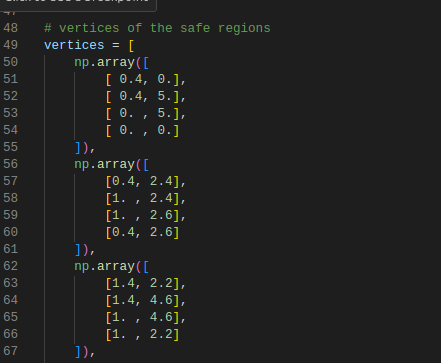
\includegraphics[width=0.5\linewidth]{imgs/2d-decompose.png}
    \end{figure}
    
    \item Với ví dụ \textbf{Motion Planning in a Maze (7.2)}, \textbf{mỗi ô trong mê cung \( 50 \times 50 \) được xem là một vùng lồi an toàn \( Q_i \)}; Mê cung được phân hoạch bằng lưới đều (grid decomposition) với các ô vuông đơn vị. Đồ thị kết nối (graph connectivity) được xác định dựa trên cấu trúc tường: hai ô kề nhau được kết nối nếu không có tường ngăn cách.

    \begin{figure}[H]
        \centering
        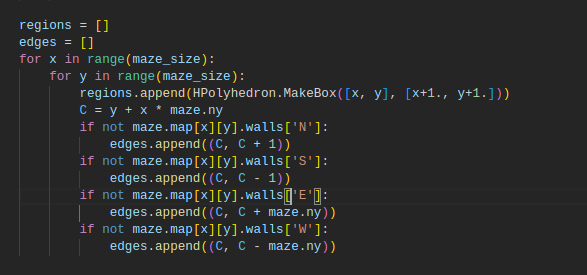
\includegraphics[width=0.5\linewidth]{imgs/maze-decompose.png}
    \end{figure}
  \end{itemize}

  \item \textbf{Ví dụ bay của quadrotor trong không gian 3D (Phần 7.3):}  
  Khi môi trường là 3D với các vật cản có dạng khối đa diện (tòa nhà, cây, tường, cửa), bài báo sử dụng \textit{phân hoạch lồi chính xác dựa trên hộp chữ nhật} (\textit{axis-aligned box decomposition}).  
  Không gian tự do được chia thành các hộp chữ nhật (convex boxes) bao quanh các vùng mở giữa các vật cản.  
  Mỗi hộp được ``thu nhỏ'' lại để bù kích thước hình học của robot (quadrotor).  
  Các hộp chồng lấn được nối với nhau thông qua điều kiện \( Q_i \cap Q_j \neq \emptyset \).

  Thuật toán chia nhỏ không gian cấu hình $Q$ thành các vùng an toàn $Q_i$ dựa trên hình dạng đa giác của các vật cản (tường, cây). 
Bán kính của quadrotor ($0.2\,\text{m}$) được tính đến bằng cách thu hẹp các vùng an toàn tương ứng.

\begin{itemize}

    \item \textbf{Xử lý các ô trong lưới (Grid Cells):}  
    Không gian làm việc được biểu diễn dưới dạng một lưới hai chiều. 
    Thuật toán duyệt qua từng ô để xác định các vùng không gian trống.

    \begin{itemize}
        \item \emph{Các phòng (Indoor Cells):}  
        Đối với mỗi ô có giá trị $\texttt{grid}[i,j] > 0.5$, một hình hộp duy nhất được tạo để bao phủ toàn bộ ô. 
        Kích thước hình hộp được thu hẹp bởi \texttt{wall\_offset} ($0.125 + \texttt{quad\_radius}$) để tránh va chạm với tường.

        \begin{lstlisting}[caption={Tạo vùng an toàn cho ô phòng trong nhà}]
regions.append(HPolyhedron.MakeBox(
    [xy[0] - (2.5 - wall_offset), xy[1] - (2.5 - wall_offset), z_min],
    [xy[0] + (2.5 - wall_offset), xy[1] + (2.5 - wall_offset), z_max]))
        \end{lstlisting}

        \item \emph{Không gian ngoài trời (Outdoor Cells):}  
        Nếu ô không có cây, một hình hộp lớn bao phủ toàn bộ vùng trống được tạo.  
        Nếu có cây, vùng xung quanh cây được chia thành \textbf{bốn hình hộp không chồng lấn} tương ứng với bốn hướng (trên, dưới, trái, phải) của cây trung tâm:

        \begin{lstlisting}[caption={Tạo vùng an toàn xung quanh cây trong không gian ngoài trời}]
regions.append(HPolyhedron.MakeBox(
                    lb, 
                    [ub[0], tree_pose[1] - 0.5, ub[2]])
                    )
regions.append(HPolyhedron.MakeBox(
                    [lb[0], tree_pose[1] - 0.5, lb[2]],
                    [tree_pose[0] - 0.5, tree_pose[1] + 0.5,
                    ub[2]]))
regions.append(HPolyhedron.MakeBox(
                    [tree_pose[0] + 0.5, tree_pose[1] - 0.5, lb[2]],
                    [ub[0], tree_pose[1] + 0.5, ub[2]]))
regions.append(HPolyhedron.MakeBox(
                    [lb[0], tree_pose[1] + 0.5, lb[2]],
                    ub))
        \end{lstlisting}
    \end{itemize}

    \item \textbf{Xử lý các khe hở trên tường (Wall Openings):}  
    Các tường được xem là vật cản, nhưng các khe hở như cửa ra vào hoặc cửa sổ lại là vùng an toàn mà quadrotor có thể đi qua.

    \begin{itemize}
        \item \emph{Cửa ra vào (Doors):}  
        Mỗi cửa được biểu diễn bằng một hình hộp hẹp, cao với kích thước đã trừ bán kính quadrotor (\texttt{door\_width}, \texttt{door\_height}).
        \item \emph{Cửa sổ (Windows):}  
        Một hoặc hai hình hộp nhỏ được tạo tại vị trí cửa sổ, xác định bởi \texttt{window\_width}, \texttt{window\_z\_min}, và \texttt{window\_z\_max}.
        \item \emph{Tường lửng (Half Walls):}  
        Sinh ra vùng trống ở phía trên hoặc bên cạnh chúng.
        \item \emph{Không có tường (No Wall):}  
        Khi hai phòng nối với nhau mà không có tường, một hình hộp lớn được tạo để kết nối hai vùng.
    \end{itemize}

    \item \textbf{Kết quả cuối cùng:}  
    Sau khi duyệt qua toàn bộ ô, cây và tường, biến \texttt{regions} chứa danh sách các hình hộp an toàn (\texttt{HPolyhedron}). 
    Tập hợp này tạo thành một \textbf{phân rã lồi chính xác} của toàn bộ không gian cấu hình bay an toàn cho quadrotor.

\end{itemize}

  \item \textbf{Ví dụ cánh tay robot bậc tự do cao (Phần 7.4 -- KUKA LBR iiwa 7-DOF):}  
  Trong không gian cấu hình bảy chiều, các vật cản khiến vùng tự do trở nên phi lồi và không thể phân hoạch chính xác.  
  Bài báo vì thế áp dụng \textit{phân hoạch lồi xấp xỉ} (\textit{approximate convex decomposition}) sử dụng thuật toán \textbf{IRIS (Iterative Regional Inflation by Semidefinite Programming)}~\cite{DeitsTedrake2014}.  
  Cụ thể, tác giả viết:
  \begin{quote}
    ``We then adopt the approximate decomposition algorithm, IRIS, from [5]; more precisely, its extension to configuration spaces with nonconvex obstacles, \texttt{IrisInConfigurationSpace}, implemented in Drake [36].''
  \end{quote}
  Phương pháp này sinh ra các đa diện lồi \( Q_i \) không va chạm quanh \textbf{các seed poses được chọn thủ công.}  
  Mỗi polytope được ``phồng'' tối đa bằng các ràng buộc nửa không gian và bài toán SDP; quá trình này được thực hiện song song cho các seed khác nhau.

  \item \textbf{Ví dụ phối hợp hai cánh tay robot (Phần 7.5 -- 14 DOF):}  
  Trong không gian 14 chiều, bài báo mở rộng cùng phương pháp IRIS ở trên.  
  Các vùng lồi cho từng cánh tay được tạo độc lập, sau đó kết hợp (theo tích Descartes hoặc hợp lồi) để tạo các vùng an toàn trong không gian cấu hình chung.  
  Đây vẫn là \textit{approximate IRIS-based convex decomposition}.
\end{itemize}


Bài báo cũng lưu ý rằng \textbf{việc gieo mầm cho quá trình này được thực hiện thủ công thông qua động học ngược}, điều này làm nổi bật chính xác vấn đề mà thuật toán VCC được thiết kế để giải quyết. Việc sử dụng IrisInConfigurationSpace để tạo ra các tập lồi cần thiết cho thấy rằng nếu không có một công cụ như vậy, khuôn khổ GCS sẽ bị giới hạn trong các môi trường đơn giản với các chướng ngại vật đa diện. Sự thành công của các phương pháp giống IRIS trong các không gian cấu hình nhiều chiều, không lồi trực tiếp cho phép ứng dụng GCS vào các robot trong thế giới thực.

\section{Appendix}

\subsection{Độ lõm theo đường đi ngắn nhất (Shortest Path Concavity – SP-Concavity)}
\label{sec:SP-Concavity}

Phương pháp SP-Concavity xác định độ lõm của mỗi đỉnh trong vùng lõm (\textit{pocket}) $\rho$ dựa trên 
\textbf{độ dài đường đi ngắn nhất} từ đỉnh đó đến đoạn cầu nối (\textit{bridge}) $\beta = (\beta^-, \beta^+)$ 
nằm trong đa giác con $P_\rho$ được tạo bởi $\beta$ và biên $\rho$.  

Trước tiên, ta chia $P_\rho$ thành ba miền $A$, $B$, và $C$ (Hình~\ref{fig:sp-concavity}).  
Đường đi ngắn nhất từ các đỉnh thuộc $A$ và $C$ đến $\beta$ tương ứng là đường ngắn nhất đến $\beta^-$ và $\beta^+$.  
Các đường này được tìm bằng cách xây dựng hai \textbf{cây tầm nhìn} (visibility trees) 
gốc tại $\beta^-$ và $\beta^+$.

Đối với các đỉnh thuộc miền $B$, đường đi ngắn nhất đến $\beta$ được tạo bởi hai phần:
\[
\pi(x, y) + \pi(y, \beta), \quad \forall y \in V^+_\beta,
\]
trong đó $V^+_\beta$ là tập các đỉnh nhìn vuông góc đến đoạn cầu $\beta$ 
(\textit{perpendicularly visible vertices}).  
Các tập $V^+_\beta$ và $V^-_\beta$ được xác định bằng cách duyệt biên $\partial B$ theo thứ tự.

Thuật toán tính SP-Concavity cho từng đỉnh được tóm tắt trong \textbf{Thuật toán~\ref{alg:sp-concavity}} 
với độ phức tạp $O(n)$, trong đó $n$ là số đỉnh của biên $\partial P_0$.  
Độ lõm của một đỉnh $v$ trong $\rho$ chính là độ dài đường đi ngắn nhất từ $v$ đến $\beta$.


\begin{algorithm}[H]
\caption{Tính khoảng cách ngắn nhất đến cầu nối $\beta$ (\texttt{Dist2Bridge}$(\beta, \rho)$)}
\label{alg:sp-concavity}
\begin{algorithmic}[1]
    \State Chia $P_\rho$ thành ba miền $A$, $B$, và $C$.
    \State Xây dựng hai cây tầm nhìn $T_1$, $T_2$ gốc tại $\beta^-$ và $\beta^+$.
    \State Tính $\pi(v, \beta)$ cho mọi $v \in A$ và $v \in C$ từ $T_1$ và $T_2$.
    \State Xác định tập $V^+_\beta$ trong miền $B$.
    \For{mỗi cặp $(v_i, v_j) \in V^+_\beta$}
        \For{mỗi $v_k$ sao cho $i < k < j$}
            \State $\pi(v_k, \beta) \gets \min\big(\pi(v_k, v_i), \pi(v_k, v_j)\big) + \pi(v, \beta)$
        \EndFor
    \EndFor
\end{algorithmic}
\end{algorithm}

\noindent

\begin{figure}[H]
    \centering
    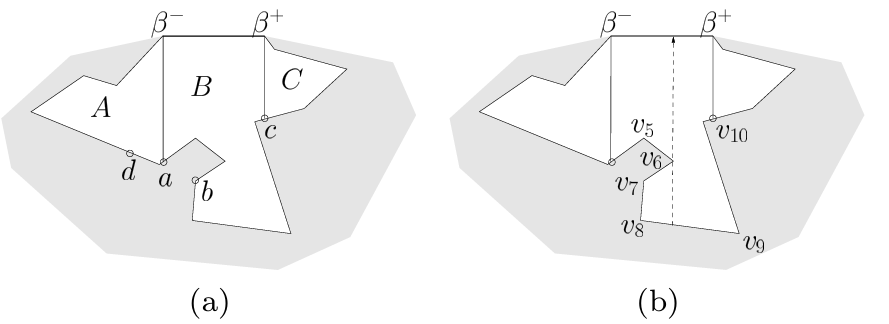
\includegraphics[width=0.7\textwidth]{imgs/sp_concavity.png}
    \caption{Minh họa chia miền $A$, $B$, $C$ và các đỉnh $V^+_\beta$, $V^-_\beta$.}
    \label{fig:sp-concavity}
\end{figure}

\newpage

\bibliographystyle{unsrtnat}
\bibliography{references}


% Assuming images are placed here; adjust positions as needed

\end{document}